\documentclass{report}
\usepackage[utf8]{inputenc}
\usepackage{float}
\usepackage[pdftex]{graphicx}
\usepackage{amsmath}
\usepackage[pdftex]{hyperref}
\usepackage{tabularx}
\DeclareGraphicsExtensions{.pdf,.jpeg,.png,.PNG}

\renewcommand{\figurename}{Imagem}

\title{Simulação de um processo de manipulação com um robô de braço duplo do tipo Yaskawa SDA10F}
\author{Pedro Miguel Loureiro Amaral}
\date{9 de Janeiro de 2022}

\begin{document}

\maketitle

\renewcommand\thesection{\arabic{section}}

\section{Introdução}

Este relatório tem por objetivo explorar a cinemática direta, inversa e diferencial de um robô de braço duplo do tipo Yaskawa SDA10F. Este robô tem um total de 15 graus de liberdade tendo uma junta colinear no tronco e em cada braço alternadamente 4 juntas colineares e 3 ortogonais.

Após definir a sua cinemática será abordado o desenvolvimento do código de uma aplicação em Matlab que mostre uma animação do movimento de um robô. Nesta animação, o robô a pegar em 2 blocos vindos de tapetes rolantes diferentes, 1 com cada braço, depois os junte simulando uma operação de colagem e finalmente rode e pouse no tapete rolante atrás. Após estas ações o robô deve rodar de novo para frente e preparar-se para pegar em novos blocos. Nesta animação também deve ser simulado o movimento dos blocos que deve acontecer linearmente enquanto estiverem nos tapetes, à exceção dos momentos em que o robô os estiver a pegar ou a pousar.

\section{Cinemática Direta}

Para começar a analisar o robô deste projeto é necessário primeiro estabelecer a cinemática direta deste. Inicialmente foi concluída a seguinte:

\begin{table}[H]
\centering
\caption{Cinemática Direta do Braço Direito}
\label{table:cinematica_direta_direito_inicial}
\begin{tabular}{ | m{1.7cm} | m{1.7cm}| m{1.7cm} | m{1.7cm} | m{1.7cm} | }
\hline
Elo i & $\theta i$ & $li$ & $di$ & $\alpha i$ \\
\hline
1 & $\theta 1$ & $LX$ & $LZ$ & $-\pi /2$ \\
\hline
2 & $\theta 2$ & $0$ & $LA$ & $\pi /2$ \\
\hline
3 & $\theta 3$ & $0$ & $0$ & $-\pi /2$ \\
\hline
4 & $\theta 4$ & $0$ & $LB$ & $\pi /2$ \\
\hline
5 & $\theta 5$ & $0$ & $0$ & $-\pi /2$ \\
\hline
6 & $\theta 6$ & $0$ & $LC$ & $\pi /2$ \\
\hline
7 & $\theta 7$ & $0$ & $0$ & $-\pi /2$ \\
\hline
8 & $\theta 8$ & $0$ & $LD$ & $0$ \\
\hline
\end{tabular}
\end{table}

 No entanto esta foi alterada de forma a criar uma junta virtual entre as juntas 0 e 1 para obter uma melhor visualização e outra entre as juntas 4 e 5 para facilitar os cálculos da cinemática inversa. Adicionalmente, para facilitar a animação foi também considerado que o robô na posição "zero hardware" encontra-se virado para x negativo. Assim sendo foram considerados os parâmetros de cinemática direta nas seguintes tabelas:

\begin{table}[H]
\centering
\caption{Cinemática Direta do Braço Direito}
\label{table:cinematica_direta_direito}
\begin{tabular}{ | m{1.7cm} | m{1.7cm}| m{1.7cm} | m{1.7cm} | m{1.7cm} | }
\hline
Elo i & $\theta i$ & $li$ & $di$ & $\alpha i$ \\
\hline
1 & $\theta 1 + \pi /2$ & $0$ & $LZ$ & $-\pi /2$ \\
\hline
1a & $- \pi /2$ & $0$ & $LX$ & $-\pi /2$ \\
\hline
2 & $\theta 2 + \pi /2$ & $0$ & $LA$ & $\pi /2$ \\
\hline
3 & $\theta 3$ & $0$ & $0$ & $-\pi /2$ \\
\hline
4 & $\theta 4$ & $0$ & $LB$ & $\pi /2$ \\
\hline
5 & $\theta 5 + \pi /2$ & $LC$ & $0$ & $0$ \\
\hline
5a & $- \pi /2$ & $0$ & $0$ & $-\pi /2$ \\
\hline
6 & $\theta 6$ & $0$ & $0$ & $\pi /2$ \\
\hline
7 & $\theta 7$ & $0$ & $0$ & $-\pi /2$ \\
\hline
8 & $\theta 8$ & $0$ & $LD$ & $0$ \\
\hline
\end{tabular}
\end{table}

\begin{table}[H]
\centering
\caption{Cinemática Direta do Braço Esquerdo}
\label{table:cinematica_direta_esquerdo}
\begin{tabular}{ | m{1.7cm} | m{1.7cm}| m{1.7cm} | m{1.7cm} | m{1.7cm} | }
\hline
Elo i & $\theta i$ & $li$ & $di$ & $\alpha i$ \\
\hline
1 & $\theta 1 + \pi /2$ & $0$ & $LZ$ & $-\pi /2$ \\
\hline
1a & $- \pi /2$ & $0$ & $LX$ & $\pi /2$ \\
\hline
2 & $\theta 2 - \pi /2$ & $0$ & $LA$ & $-\pi /2$ \\
\hline
3 & $\theta 3$ & $0$ & $0$ & $\pi /2$ \\
\hline
4 & $\theta 4$ & $0$ & $LB$ & $-\pi /2$ \\
\hline
5 & $\theta 5 - \pi /2$ & $LC$ & $0$ & $0$ \\
\hline
5a & $\pi /2$ & $0$ & $0$ & $\pi /2$ \\
\hline
6 & $\theta 6$ & $0$ & $0$ & $-\pi /2$ \\
\hline
7 & $\theta 7$ & $0$ & $0$ & $+\pi /2$ \\
\hline
8 & $\theta 8$ & $0$ & $LD$ & $0$ \\
\hline
\end{tabular}
\end{table}

\section{Cinemática Inversa}

Uma das formas para mover os end-effectors do robô é através da sua cinemática inversa. No entanto este robô tem 15 graus de liberdade, 7 em cada braço e 1 no tronco, o que o faz infinitamente redundante. Assim de forma a ser possível calcular um número finito de soluções com a cinemática inversa foram fixadas 3 juntas, a junta 0 dado que influencia o movimento dos 2 braços e a junta 3 de cada um dos braços dado que fixar uma junta ortogonal ou a junta 1 iria diminuir o espaço de trabalho e a 5 e a 7 são convenientes para definir a orientação dos end-effectors.

Após reduzir cada braço a 6 graus de liberdade foi usado o conceito de punho esférico de modo a calcular as soluções. Um punho esférico existe quando as 3 últimas juntas são colinear-ortogonal-colinear e o centro do referencial das 3 juntas é o mesmo. Dado que inicialmente o robô não tinha a antepenúltima junta com o centro igual às restantes 2 criou-se a junta virtual 5a referida na secção da cinemática direta de modo a efetuar uma translação dessa junta para coincidir com as outras 2.

Considerando que o último elo deve estar na direção vertical no sentido para baixo (y negativo), então é possível calcular os valores referentes à translação da matriz de transformação desde a junta 0 até à 5a da seguinte forma:
\begin{equation}
    \begin{cases}
      Pwx = x\\
      Pwy = y\\
      Pwz = z - LD
    \end{cases}
\end{equation}

Excluindo as últimas 3 juntas, a matriz de transformação resulta da multiplicação das restantes matrizes. Como $\theta 1$ e $\theta 3$ estão fixados a 0 encontramos então as seguintes expressões para as coordenadas de Pw no braço direito:

\begin{equation}
    \begin{cases}
      Pwx = -LX -LC*c2*c5*s3 - LB*c2*s3 - LC*s5*c2*c3\\
      Pwy = LA + LB*c3 - LC*s5*s3 + LC*c5*c3\\
      Pwz = LZ + LB*s2*s3 + LC*s5*s2*c3 + LC*c5*s2*s3
     \end{cases}
\end{equation}

Este sistema de equações tem 3 incógnitas que são o $\theta 2$, $\theta 3$ e $\theta 5$. Através da divisão de Pwz por Pwx é possível deduzir que:

\begin{equation}
    \theta 2 = arctan(\frac{(Pwz-LZ)*sign(LB*s3 + LC*s5*c3 + LC*c5*s3)}{(-Pwx-LX)*sign(LB*s3 + LC*s5*c3 + LC*c5*s3))}
\end{equation}

É também possível deduzir apartir da soma de todos os quadrados que:

\begin{equation}
    \theta 5 = \pm arccos(\frac{(-Pwx-LX)^2+(Pwy-LA)^2+(Pwz-LZ)^2-LB^2-LC^2}{2*LB*LC}
\end{equation}

É ainda possível, através da equação de Pwy e da solução de $acos(\theta)+bsin(\theta)=c$, deduzir que:

\begin{equation}
    \theta 3 = 2*arctan(\frac{-LC*s5\pm \sqrt{LB^2+LC^2+2*LB*LC*c5-(Pwy-LA)^2}}{LB+LC*c5+Pwy-LA}
\end{equation}

Com os ângulos anteriores definidos faltam então os pertencentes ao punho esférico. Para isso é necessário calcular a matriz de transformação referente a esses 3 ângulos. Esta pode ser calculada com a multiplicação $A6*A7*A8$ resultando nos 3 ângulos necessários como as 3 incógnitas. Numericamente, após calcular $\theta 2$, $\theta 3$ e $\theta 5$ e sabendo a posição e orientação do end-effector, também pode ser calculada da seguinte forma:

\begin{equation}
    0T8 = 0T5a * 5T8 \Leftrightarrow 5T8 = (0T5a)^{-1}
    * 0T8
\end{equation}

Consequentemente, a partir de a3x e a3y podemos concluir:

\begin{equation}
    \begin{cases}
      a3x = -c6*s7\\
      a3y = -s6*s7\\
     \end{cases} \Leftrightarrow \theta 6 = arctan(\frac{\mp a3y}{\mp a3x})
\end{equation}

Considerando que $a3x^2 + a3y^2 = s5^2$ e que $a3z=c5$ então para $\theta 7$ temos:

\begin{equation}
    \theta 7 = arctan(\frac{\pm \sqrt{a3x^2 + a3y^2}}{a3z})
\end{equation}

Finalmente de s3z e n3z podemos concluir:

\begin{equation}
    \begin{cases}
      s3z = -s7*s8\\
      n3z = s7*c8\\
     \end{cases} \Leftrightarrow \theta 8 = arctan(\frac{\pm s3z}{\mp n3z})
\end{equation}

Para o braço esquerdo foi efetuado um processo semelhante sendo as equações bastante parecidas com algumas trocas de sinais.

\section{Cinemática Diferencial}

A segunda forma de calcular os movimentos do robô é através da cinemática diferencial deste. Este método permite um melhor controlo da trajetória do end-effector do robô mas apresenta alguma incerteza. Sendo $r = [x$ $y$ $z$ $\phi$ $\theta$ $\psi]$ representando a posição e orientação do end-effector, $q = [\theta 2$ $\theta 3$ $\theta 5$ $\theta 6$ $\theta 7$ $\theta 8]$ representando os ângulos de junta relevantes e J o jacobiano da função de transformação, para calcular o jacobiano de cada braço do robô foram derivadas em relação a $\theta 2$, $\theta 3$, $\theta 5$, $\theta 6$, $\theta 7$ e $\theta 8$ as seguintes equações:

\begin{equation}
    \begin{cases}
      x = T(1,4)\\
      y = T(2,4)\\
      z = T(3,4)\\
      \phi = arctan(\frac{T(2,1)}{T(1,1)})\\
      \theta = arctan(-T(3,1)/\sqrt{T(1,1)^2+T(2,1)^2})\\
      \psi = arctan(T(3,2)/T(3,3))
     \end{cases},T \Rightarrow \text{matriz de transformação}
\end{equation}

É de notar que quando a cinemática diferencial é usada, $\theta$ e a sua derivada têm sempre o valor 0 implicando que o seu cosseno é sempre superior a 0, validando o uso das equações acima para $\phi$ e $\psi$.

Dada a definição de jacobiano, segue-se a seguinte equação:

\begin{equation}
    dr = J * dq
\end{equation}

Isto também significa que usando o Jacobiano Inverso:

\begin{equation}
    dq = J^{-1} * dr
\end{equation}

Sendo dr constante podemos considerar dr como a alteração da posição e orientação do end-effector. Ao multiplicar o jacobiano inverso por este vetor encontramos assim a evolução dos ângulos de juntas para o movimento do end-effector indicado no vetor. Este método permite assim que sejam efetuados movimentos lineares.
 
\section{Principais Funções}

\begin{itemize}
    \item InitRobot: desenha o Robô no ambiente de simulação e retorna os "handlers" gráficos de cada braço.
    \item invkinL, invkinR: cálculo da cinemática inversa do braço esquerdo e do direito, respetivamente. Caso os resultados sejam todos imaginários ou ultrapassem os limites das juntas, o que significa que o destino está fora do espaço de trabalho, estas funções devolvem uma lista vazia. Caso existam várias soluções possíveis é escolhida a com menor soma dos ângulos.
    \item jacobianL, jacobianR: devolvem a matriz do jacobiano do braço esquerdo e direito, respetivamente.
    \item jacobianLInv, jacobianRInv: devolvem a matriz do jacobiano inverso do braço esquerdo e direito, respetivamente. Caso a matriz do jacobiano não tenha inversa, devolvem NaN.
    \item CalculateRobotMotion: calcula e devolve a superhipermatriz com todas as transformações geométricas através das matrizes de DH para as diversas configurações. Opcionalmente, desenha o caminho do end-effector.
    \item JacobianMotion: calcula e adiciona as transformações geométricas de um determinado movimento através de cinemática diferencial à superhipermatriz com todas as transformações geométricas. Se o jacobiano inverso for impossível de calcular ou os resultados ultrapassarem os limites das juntas emite uma mensagem de erro e fecha o programa.
    \item InverseMotion: calcula e adiciona as transformações geométricas de um determinado movimento através de cinemática inversa à superhipermatriz com todas as transformações geométricas.
    \item TP2Animation: função principal do programa, usa todas as funções anteriores para fazer os cálculos necessários para obter o caminhos dos end-effectors e no fim mostra a animação dos movimentos dos braços dos robôs incluindo o gripper e dos blocos. Adicionalmente também mostra uma mensagem de erro e fecha o programa quando as funções da cinemática inversa não devolvem uma solução.
\end{itemize}

\section{Diagrama de Funcionamento Geral}

\begin{figure}[H]
   \centering
   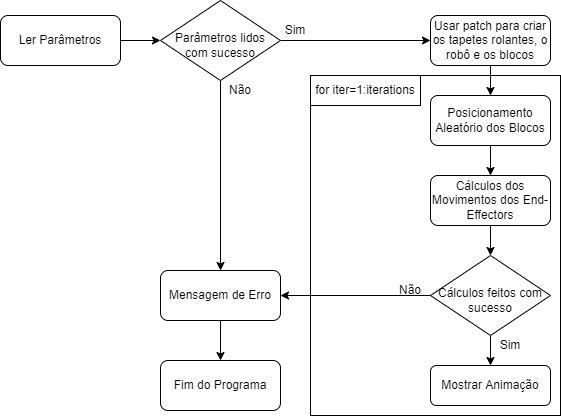
\includegraphics[width=4.5in]{diagram.png}
   \label{fig:figuras}
   \caption{Diagrama de Funcionamento Geral do Programa}
\end{figure}

\section{Execução do Programa}

Para executar o programa o utilizador deve chamar a função TP2Animation que tem 2 parâmetros: plotPath que decide que o caminho dos end-effectors deve ser representado antes do movimento e iterations que decide o número de vezes que a animação ocorre. Um exemplo pode ser encontrado no ficheiro "main.m".

\section{Conclusão}

\quad Concluindo, foram cumpridos todos os requisitos do projeto tendo sido possível obter a cinemática direta, inversa e diferencial do robô e sendo possível observar na animação o seu uso para animar o movimento de um robô a mover blocos. Como ponto extra, os blocos foram apanhados das primeiros tapetes com orientações e posições aleatórias.

Por fim, segue-se o vídeo demonstrativo: \url{https://www.youtube.com/watch?v=QfRQ9jFAsH4}.

\end{document}
